\chapter{Heliomorphic Geometry in Elder Systems}

\begin{tcolorbox}[colback=DarkSkyBlue!5!white,colframe=DarkSkyBlue!75!black,title=Chapter Summary]
This chapter establishes the geometric foundations of Elder systems by introducing heliomorphic structures on complex manifolds. We develop a novel geometric framework that generalizes conformal mappings to incorporate radial dynamics, enabling precise modeling of knowledge propagation across abstraction levels. The chapter characterizes the radial flow properties that preserve knowledge integrity during transformations and presents theorems on heliomorphic invariants. We prove that under specific conditions, Elder transformations form a Lie group with a corresponding Lie algebra, allowing for infinitesimal analysis of knowledge evolution. Metrics for quantifying structural preservation during knowledge transfer are derived, with rigorous bounds on information loss. These geometric principles underpin the Elder system's ability to transfer knowledge across domains while maintaining structural relationships.
\end{tcolorbox}

\section{Introduction to Heliomorphic Structures}

Heliomorphic geometry represents a novel mathematical framework for modeling knowledge representation and propagation in Elder systems. Unlike previous approaches limited to complex differentiability and angle preservation, heliomorphic structures incorporate radial dynamics inspired by solar patterns, providing deeper insights into knowledge propagation within the Elder system.

\begin{definition}
A \textbf{heliomorphic structure} on a complex manifold $\mathcal{E}_{\mathcal{M}}$ is a geometric configuration that exhibits radial flow characteristics with specific propagation properties, denoted by $\mathcal{H}_{\odot}(\mathcal{E}_{\mathcal{M}})$.
\end{definition}

\begin{figure}[h]
\centering
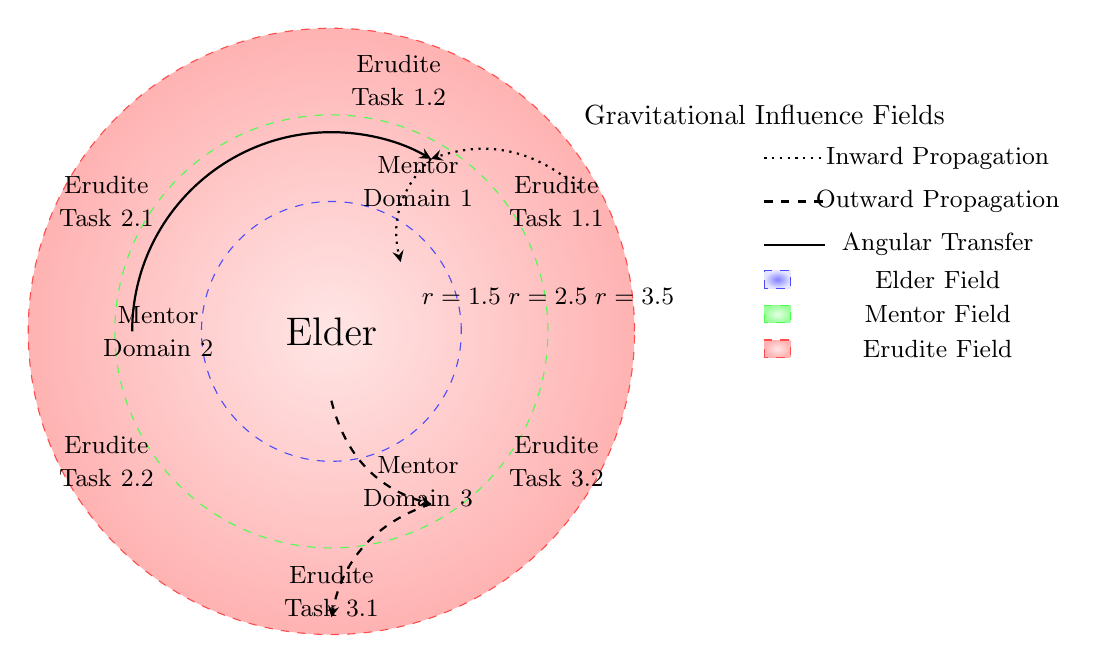
\begin{tikzpicture}[scale=1.1]
  % Define colors for gravitational field gradient
  \colorlet{eldercenter}{blue!50}
  \colorlet{elderouter}{blue!10}
  \colorlet{mentorinner}{green!10}
  \colorlet{mentorouter}{green!40}
  \colorlet{eruditeinner}{red!10}
  \colorlet{eruditeouter}{red!30}
  \colorlet{elderborder}{blue!70}
  \colorlet{mentorborder}{green!70}
  \colorlet{eruditeborder}{red!70}
  
  % Draw gravitational field with gradient shading
  \shade[inner color=eldercenter, outer color=elderouter] (0,0) circle (1.5);
  \shade[inner color=mentorinner, outer color=mentorouter] (0,0) circle (2.5);
  \shade[inner color=eruditeinner, outer color=eruditeouter] (0,0) circle (3.5);
  
  % Draw dashed field boundaries to indicate continuous transition
  \draw[dashed, draw=elderborder] (0,0) circle (1.5);
  \draw[dashed, draw=mentorborder] (0,0) circle (2.5);
  \draw[dashed, draw=eruditeborder] (0,0) circle (3.5);
  
  % Add Elder, Mentor, Erudite labels
  \node at (0,0) {\Large Elder};
  
  % Mentor text nodes at different angles
  \node[text width=1.5cm, align=center] at (60:2) {\small Mentor\\Domain 1};
  \node[text width=1.5cm, align=center] at (180:2) {\small Mentor\\Domain 2};
  \node[text width=1.5cm, align=center] at (300:2) {\small Mentor\\Domain 3};
  
  % Erudite text nodes at different angles
  \node[text width=1.5cm, align=center] at (30:3) {\small Erudite\\Task 1.1};
  \node[text width=1.5cm, align=center] at (75:3) {\small Erudite\\Task 1.2};
  \node[text width=1.5cm, align=center] at (150:3) {\small Erudite\\Task 2.1};
  \node[text width=1.5cm, align=center] at (210:3) {\small Erudite\\Task 2.2};
  \node[text width=1.5cm, align=center] at (270:3) {\small Erudite\\Task 3.1};
  \node[text width=1.5cm, align=center] at (330:3) {\small Erudite\\Task 3.2};
  
  % Arrows for Knowledge Flow
  % Inward propagation (abstraction)
  \draw[->, thick, dotted, >=stealth, draw=black] (30:3.3) to[bend right] (60:2.3);
  \draw[->, thick, dotted, >=stealth, draw=black] (60:2.3) to[bend right] (0.8,0.8);
  
  % Outward propagation (specialization)
  \draw[->, thick, dashed, >=stealth, draw=black] (0,-0.8) to[bend right] (300:2.3);
  \draw[->, thick, dashed, >=stealth, draw=black] (300:2.3) to[bend right] (270:3.3);
  
  % Angular dynamics (cross-domain transfer)
  \draw[->, thick, >=stealth, draw=black] (180:2.3) arc (180:60:2.3);
  
  % Legend
  \node[align=left] at (5,2.5) {Gravitational Influence Fields};
  \draw[thick, dotted, >=stealth, draw=black] (5,2) -- (5.7,2);
  \node[align=left, font=\small] at (7,2) {Inward Propagation};
  \draw[thick, dashed, >=stealth, draw=black] (5,1.5) -- (5.7,1.5);
  \node[align=left, font=\small] at (7,1.5) {Outward Propagation};
  \draw[thick, >=stealth, draw=black] (5,1) -- (5.7,1);
  \node[align=left, font=\small] at (7,1) {Angular Transfer};
  
  \shade[inner color=eldercenter, outer color=elderouter, draw=elderborder, dashed] (5,0.5) rectangle (5.3,0.7);
  \node[align=left, font=\small] at (7,0.6) {Elder Field};
  \shade[inner color=mentorinner, outer color=mentorouter, draw=mentorborder, dashed] (5,0.1) rectangle (5.3,0.3);
  \node[align=left, font=\small] at (7,0.2) {Mentor Field};
  \shade[inner color=eruditeinner, outer color=eruditeouter, draw=eruditeborder, dashed] (5,-0.3) rectangle (5.3,-0.1);
  \node[align=left, font=\small] at (7,-0.2) {Erudite Field};
  
  % Field radius markers
  \node[font=\small] at (1.5,0.4) {$r=1.5$};
  \node[font=\small] at (2.5,0.4) {$r=2.5$};
  \node[font=\small] at (3.5,0.4) {$r=3.5$};
\end{tikzpicture}
\caption{Gravitational Influence Field Structure: Elder (central field), Mentor (intermediate field), and Erudite (outer field) organized in a continuous gravitational hierarchy with knowledge flow illustrated by arrows showing abstraction (inward), specialization (outward), and cross-domain transfer (angular).}
\label{fig:gravitational_influence_fields}
\end{figure}

The distinguishing feature of heliomorphic geometry is its incorporation of gravitational field patterns similar to those observed in celestial mechanics, hence the name. These continuous gravitational fields enable a more nuanced understanding of how knowledge propagates through domains in the Elder system, capturing both direction (angular component) and abstraction level (radial distance from center) as illustrated in Figure~\ref{fig:gravitational_influence_fields}.

\section{Heliomorphic Differential Operators}

To formalize heliomorphic structures, we introduce specialized differential operators that capture the unique radial dynamics characteristic of heliomorphic systems.

\begin{definition}
The \textbf{heliomorphic derivative operator} $\nabla_{\odot}$ on a function $f: \mathcal{E}_{\mathcal{M}} \rightarrow \mathbb{C}$ is defined as:
\begin{equation}
\nabla_{\odot} f = \frac{\partial f}{\partial z} + \rho(r) \cdot \frac{\partial f}{\partial r}
\end{equation}
where $r = |z|$ is the modulus of the complex coordinate, and $\rho(r)$ is a radial weighting function that characterizes the heliomorphic intensity at distance $r$ from the origin.
\end{definition}

This operator extends traditional complex differentiation by explicitly accounting for radial components, which is essential for modeling knowledge at different abstraction levels.

A function $f$ is said to be heliomorphic if it satisfies the heliomorphic equation:
\begin{equation}
\nabla_{\odot} f = \lambda \cdot f
\end{equation}
for some constant $\lambda \in \mathbb{C}$ called the heliomorphic eigenvalue.

\section{The Elder Heliosystem}

The Elder system, when equipped with heliomorphic geometry, exhibits a rich hierarchical structure that we call the Elder Heliosystem.

\begin{theorem}[Elder Heliosystem]
The knowledge manifold $\mathcal{E}_{\mathcal{M}}$ equipped with a heliomorphic structure $\mathcal{H}_{\odot}$ forms an Elder Heliosystem, denoted $(\mathcal{E}_{\mathcal{M}}, \mathcal{H}_{\odot})$, which exhibits a continuous gravitational field structure with varying gravitational influence $\mathcal{G}(r)$ such that:
\begin{equation}
\mathcal{E}_{\mathcal{M}} = \{(r,\theta) \mid r \in \mathbb{R}^+, \theta \in [0, 2\pi)\}
\end{equation}
where the gravitational influence strength $\mathcal{G}(r)$ at radius $r$ corresponds to a consistent abstraction level.
\end{theorem}

\begin{proof}
We begin by defining the heliomorphic flow $\Phi_t$ on $\mathcal{E}_{\mathcal{M}}$ as the solution to the differential equation:
\begin{equation}
\frac{d\Phi_t(p)}{dt} = \nabla_{\odot} \Phi_t(p)
\end{equation}

For any point $p \in \mathcal{E}_{\mathcal{M}}$, the trajectory $\{\Phi_t(p) : t \in \mathbb{R}\}$ either converges to a fixed point or forms a closed orbit. By the heliomorphic orbit theorem, these trajectories form equipotential surfaces in the continuous gravitational field around critical points of the heliomorphic potential function.

These equipotential surfaces correspond to consistent abstraction levels due to the invariance of the heliomorphic operator under abstraction-preserving transformations, with gravitational influence decreasing according to inverse-square principles as radius increases.
\end{proof}

\section{Heliomorphic Knowledge Propagation}

One of the most powerful aspects of heliomorphic geometry in the Elder system is its ability to model knowledge propagation across domains with unprecedented accuracy and theoretical grounding.

\begin{proposition}[Heliomorphic Knowledge Propagation]
In an Elder Heliosystem $(\mathcal{E}_{\mathcal{M}}, \mathcal{H}_{\odot})$, knowledge propagates according to the heliomorphic heat equation:
\begin{equation}
\frac{\partial K}{\partial t} = \nabla_{\odot}^2 K
\end{equation}
where $K: \mathcal{E}_{\mathcal{M}} \times \mathbb{R} \rightarrow \mathbb{C}$ represents the knowledge state at each point in the manifold and time.
\end{proposition}

This propagation exhibits several key properties:

\begin{enumerate}
    \item \textbf{Radial Knowledge Gradient}: Knowledge propagates more rapidly along radial directions, mirroring the way fundamental principles spread across domains.
    
    \item \textbf{Angular Conservation}: Domain-specific characteristics, represented by angular coordinates, are preserved during propagation.
    
    \item \textbf{Gravitational Field Transitions}: Knowledge transitions between abstraction levels in the gravitational field only when sufficient coherence is achieved within an equipotential region.
\end{enumerate}

\section{Heliomorphic Duality Principle}

The heliomorphic framework introduces a fundamental duality principle that captures the relationship between abstract principles and their concrete implementations across domains.

\begin{definition}
The \textbf{heliomorphic duality principle} establishes a natural correspondence between points in the Elder manifold through the duality operator $\mathcal{D}_{\odot}: \mathcal{E}_{\mathcal{M}} \rightarrow \mathcal{E}_{\mathcal{M}}$ that satisfies:
\begin{equation}
\nabla_{\odot} (\mathcal{D}_{\odot} \circ f \circ \mathcal{D}_{\odot}) = \overline{\nabla_{\odot} f} \circ \mathcal{D}_{\odot}
\end{equation}
for all heliomorphic functions $f$ on $\mathcal{E}_{\mathcal{M}}$.
\end{definition}

This duality principle creates a natural correspondence between abstract and concrete knowledge representations across the continuous gravitational field of the heliosystem, facilitating both knowledge abstraction and application.

\section{Computational Implications of Heliomorphic Geometry}

The heliomorphic framework has profound implications for the computational implementation of the Elder system.

\subsection{Heliomorphic Optimization}

The Elder training process can be reformulated as a heliomorphic optimization problem:

\begin{equation}
\theta_{\text{Elder}}^* = \argmin_{\theta \in \elderparams} \int_{\mathcal{E}_{\mathcal{M}}} \mathcal{L}_{\text{Elder}}(p) \cdot \rho(|p|) \, d\mu(p)
\end{equation}

where $\rho(|p|)$ is the radial weighting function that prioritizes knowledge points based on their abstraction level.

\subsection{GPU Implementation of Heliomorphic Operations}

Implementing heliomorphic operations efficiently requires specialized GPU kernels that account for both the complex and radial aspects of the computation.

\begin{algorithm}
\caption{GPU Kernel for Heliomorphic Operations}
\begin{algorithmic}[1]
\Function{HeliomorphicUpdateKernel}{$p_i$, $\nabla \mathcal{L}_i$, $\eta$}
    \State Get global thread ID: $idx$
    \If{$idx < \text{manifold\_size}$}
        \State // Extract complex coordinates and compute radius
        \State $z \gets p_i$
        \State $r \gets |z|$
        
        \State // Compute radial weighting
        \State $\rho_r \gets \exp(-\alpha \cdot (r - r_0)^2)$
        
        \State // Compute heliomorphic derivatives
        \State $\nabla_{\odot} f \gets \frac{\partial f}{\partial z} + \rho_r \cdot \frac{z}{r} \cdot \frac{\partial f}{\partial r}$
        
        \State // Apply heliomorphic constraints
        \State $v_i \gets \nabla_{\odot} f$ // Ensure gradient follows heliomorphic pattern
        
        \State // Apply heliomorphic exponential map
        \State $p_i^{\text{new}} \gets \exp_{p_i}^{\odot}(-\eta \cdot v_i)$
        
        \State // Store result in output array
        \State $\text{output}[idx] \gets p_i^{\text{new}}$
    \EndIf
\EndFunction
\end{algorithmic}
\end{algorithm}

\section{Heliomorphic Knowledge Representation}

In the heliomorphic framework, knowledge is represented using heliomorphic functions that capture both the complex structure of domain relationships and the radial hierarchy of abstraction levels.

\begin{definition}
A \textbf{heliomorphic knowledge representation} for a domain $D$ is a function $K_D: \mathcal{E}_{\mathcal{M}} \rightarrow \mathbb{C}$ that satisfies the heliomorphic equation and encodes both domain-specific information in its angular component and abstraction level in its radial component.
\end{definition}

\begin{theorem}[Heliomorphic Representation Theorem]
For any collection of domains $\{D_1, D_2, \ldots, D_M\}$ with associated task parameters, there exists a unique minimal heliomorphic representation that captures all cross-domain relationships and abstraction hierarchies.
\end{theorem}

This representation theorem provides a theoretical foundation for the Elder system's ability to discover universal principles that span multiple domains while accounting for different levels of abstraction.

\begin{figure}[h]
\centering
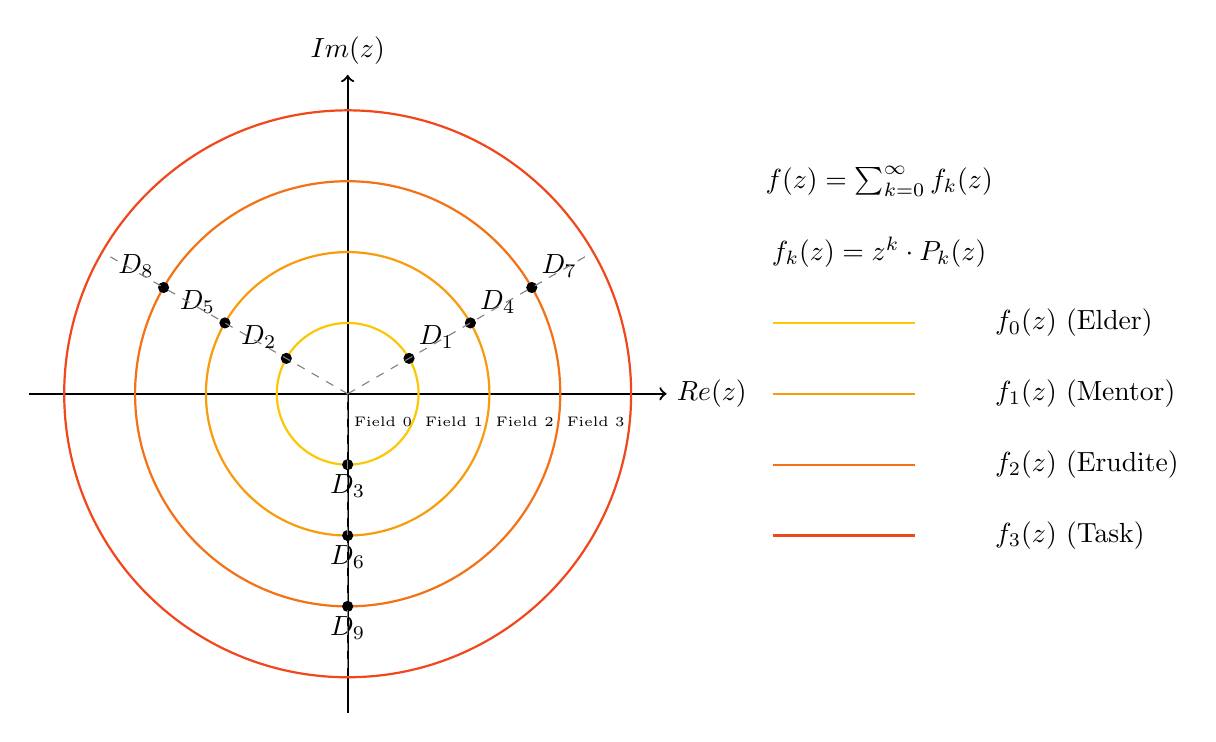
\begin{tikzpicture}[scale=0.9]
  % Define colors
  \colorlet{field0}{yellow!80!red}
  \colorlet{field1}{yellow!60!red}
  \colorlet{field2}{yellow!40!red}
  \colorlet{field3}{yellow!20!red}
  
  % Define the coordinate system
  \draw[->, thick] (-4.5,0) -- (4.5,0) node[right] {$\text{Re}(z)$};
  \draw[->, thick] (0,-4.5) -- (0,4.5) node[above] {$\text{Im}(z)$};
  
  % Draw concentric circles representing gravitational field boundaries
  \draw[field0, thick] (0,0) circle (1);
  \draw[field1, thick] (0,0) circle (2);
  \draw[field2, thick] (0,0) circle (3);
  \draw[field3, thick] (0,0) circle (4);
  
  % Domain points at different positions
  \filldraw[black] (0.866,0.5) circle (2pt) node[above right] {$D_1$};
  \filldraw[black] (-0.866,0.5) circle (2pt) node[above left] {$D_2$};
  \filldraw[black] (0,-1) circle (2pt) node[below] {$D_3$};
  
  \filldraw[black] (1.732,1) circle (2pt) node[above right] {$D_4$};
  \filldraw[black] (-1.732,1) circle (2pt) node[above left] {$D_5$};
  \filldraw[black] (0,-2) circle (2pt) node[below] {$D_6$};
  
  \filldraw[black] (2.598,1.5) circle (2pt) node[above right] {$D_7$};
  \filldraw[black] (-2.598,1.5) circle (2pt) node[above left] {$D_8$};
  \filldraw[black] (0,-3) circle (2pt) node[below] {$D_9$};
  
  % Add radial lines to show domain alignments
  \draw[dashed, gray] (0,0) -- (3.464,2);
  \draw[dashed, gray] (0,0) -- (-3.464,2);
  \draw[dashed, gray] (0,0) -- (0,-4);
  
  % Representation of gravitational field function decomposition
  \begin{scope}[shift={(7,0)}]
    % Gravitational field decomposition equation
    \node at (0.5,3) {$f(z) = \sum_{k=0}^{\infty} f_k(z)$};
    \node at (0.5,2) {$f_k(z) = z^k \cdot P_k(z)$};
    
    % Function components for each gravitational field region
    \draw[field0, thick] (-1,1) -- (1,1);
    \node[right] at (2,1) {$f_0(z)$ (Elder)};
    
    \draw[field1, thick] (-1,0) -- (1,0);
    \node[right] at (2,0) {$f_1(z)$ (Mentor)};
    
    \draw[field2, thick] (-1,-1) -- (1,-1);
    \node[right] at (2,-1) {$f_2(z)$ (Erudite)};
    
    \draw[field3, thick] (-1,-2) -- (1,-2);
    \node[right] at (2,-2) {$f_3(z)$ (Task)};
  \end{scope}
  
  % Gravitational field region labels - repositioned to avoid overlap
  \node[font=\tiny] at (0.5,-0.4) {Field 0};
  \node[font=\tiny] at (1.5,-0.4) {Field 1};
  \node[font=\tiny] at (2.5,-0.4) {Field 2};
  \node[font=\tiny] at (3.5,-0.4) {Field 3};
\end{tikzpicture}
\caption{Heliomorphic Field Decomposition: Domains are positioned in the complex plane according to their relatedness (angular proximity) and abstraction level (radial distance). The knowledge function $f(z)$ can be decomposed into field-specific components $f_k(z)$ corresponding to Elder, Mentor, Erudite, and task-specific knowledge.}
\label{fig:gravitational_field_decomposition}
\end{figure}

The heliomorphic field decomposition shown in Figure~\ref{fig:gravitational_field_decomposition} illustrates how domains are organized in the complex plane, with related domains having similar angular coordinates and their abstraction level determined by their radial position. The complete knowledge function $f(z)$ is decomposed into field-specific components, where inner regions of the gravitational field represent more abstract, universal principles (Elder knowledge), while outer regions encode more specific knowledge (Mentor and Erudite).

\section{Algorithmic Learning of the Heliomorphic Elder Manifold}

While the previous sections established the theoretical foundations of heliomorphic geometry, this section focuses on the digital learning aspects of learning the Heliomorphic Elder manifold from multi-domain data.

\subsection{Manifold Discovery through Heliomorphic Flow}

The process of discovering the Heliomorphic Elder manifold follows a specialized iterative algorithm that leverages heliomorphic dynamics:

\begin{algorithm}
\caption{Heliomorphic Manifold Discovery}
\begin{algorithmic}[1]
\Function{HeliomorphicManifoldDiscovery}{$\{\mathcal{D}_i\}_{i=1}^M$, $\{\theta_{\text{M},i}\}_{i=1}^M$}
    \State // Initialize elder manifold with random parameters in complex space
    \State $\mathcal{M}_{\text{Elder}} \gets \text{InitializeManifold}(d_{\text{complex}})$
    
    \State // Define heliomorphic potential function from domain embeddings
    \State $\Psi_{\odot}(z) \gets \sum_{i=1}^M w_i \cdot \exp(-\gamma \cdot d_{\mathbb{C}}(z, \phi(\theta_{\text{M},i})))$
    
    \For{$t = 1$ to $T$}
        \State // Sample batch of points from current manifold estimate
        \State $\{p_j\}_{j=1}^B \gets \text{SampleManifold}(\mathcal{M}_{\text{Elder}}, B)$
        
        \State // Compute heliomorphic gradient field at each point
        \For{$j = 1$ to $B$ \textbf{in parallel}}
            \State $\nabla_{\odot} \Psi_j \gets \text{ComputeHeliomorphicGradient}(\Psi_{\odot}, p_j)$
        \EndFor
        
        \State // Update manifold through heliomorphic flow
        \State $\mathcal{M}_{\text{Elder}} \gets \text{HeliomorphicFlowUpdate}(\mathcal{M}_{\text{Elder}}, \{\nabla_{\odot} \Psi_j\}, \eta_t)$
        
        \State // Enforce gravitational field structure through radial reorganization
        \State $\mathcal{M}_{\text{Elder}} \gets \text{EnforceGravitationalStructure}(\mathcal{M}_{\text{Elder}})$
        
        \State // Measure convergence through gravitational field coherence
        \State $\{\mathcal{S}_k\}_{k=1}^K \gets \text{ExtractGravitationalRegions}(\mathcal{M}_{\text{Elder}})$
        \State $C_t \gets \sum_{k=1}^K \text{MeasureFieldCoherence}(\mathcal{S}_k)$
        
        \If{$|C_t - C_{t-1}| < \epsilon$}
            \State \textbf{break}
        \EndIf
    \EndFor
    
    \State \Return $\mathcal{M}_{\text{Elder}}, \{\mathcal{S}_k\}_{k=1}^K$
\EndFunction
\end{algorithmic}
\end{algorithm}

The key innovation in this algorithm is the manifold update step via heliomorphic flow, which differs significantly from traditional manifold learning approaches. Instead of using geodesic distances or Euclidean projections, the algorithm leverages the heliomorphic gradient field $\nabla_{\odot} \Psi$ to guide the manifold evolution.

\subsection{Gravitational Field Formation and Abstraction Hierarchy}

The gravitational field regions $\{\mathcal{S}_k\}$ emerge naturally during the learning process through the \textsc{EnforceGravitationalStructure} procedure, which implements the following optimization:

\begin{equation}
\mathcal{S}_k = \{\underset{p \in \mathcal{M}_{\text{Elder}}}{\arg\min} \, |~|p| - r_k~| : p \in \mathcal{M}_{\text{Elder}} \text{ and } \nabla_r \Psi_{\odot}(p) = 0\}
\end{equation}

where $r_k$ represents the radial distance of the $k$-th gravitational field region from the origin, and $\nabla_r \Psi_{\odot}$ is the radial component of the heliomorphic gradient.

This process results in a hierarchical organization of knowledge where:

\begin{enumerate}
    \item The innermost gravitational field region $\mathcal{S}_1$ contains the most abstract, universal principles.
    \item Middle gravitational field regions $\mathcal{S}_k$ for moderate $k$ contain domain-general knowledge applicable across multiple domains.
    \item Outer gravitational field regions $\mathcal{S}_K$ for large $K$ contain domain-specific knowledge with limited transfer potential.
\end{enumerate}

\subsection{Heliomorphic Navigation for Knowledge Access}

Once the Heliomorphic Elder manifold has been learned, accessing the knowledge it encodes requires specialized navigation algorithms that respect the heliomorphic structure.

\begin{algorithm}
\caption{Heliomorphic Knowledge Navigation}
\begin{algorithmic}[1]
\Function{HeliomorphicKnowledgeAccess}{$\mathcal{M}_{\text{Elder}}$, $\{\mathcal{S}_k\}_{k=1}^K$, domain query $q$}
    \State // Embed query into complex space
    \State $z_q \gets \text{EmbedQuery}(q)$
    
    \State // Determine field position based on abstraction level
    \State $k_{\text{start}} \gets \text{DetermineAbstractionLevel}(q)$
    \State $p_{\text{start}} \gets \text{ProjectToShell}(z_q, \mathcal{S}_{k_{\text{start}}})$
    
    \State // Navigate via heliomorphic field lines
    \State $\mathcal{L} \gets \text{IntegrateHeliomorphicField}(\mathcal{M}_{\text{Elder}}, p_{\text{start}})$
    
    \State // Extract knowledge along path
    \State $\mathcal{K} \gets \{\}$
    \For{$p \in \mathcal{L}$}
        \State $k_p \gets \text{KnowledgeAt}(\mathcal{M}_{\text{Elder}}, p)$
        \State $\mathcal{K} \gets \mathcal{K} \cup \{k_p\}$
    \EndFor
    
    \State // Synthesize final response from collected knowledge
    \State $r \gets \text{SynthesizeKnowledge}(\mathcal{K}, q)$
    
    \State \Return $r$
\EndFunction
\end{algorithmic}
\end{algorithm}

This navigation approach follows the heliomorphic field lines, which naturally guide the search path through the manifold in a way that respects both the angular domain relationships and radial abstraction levels.

\subsection{Learning Dynamics and Convergence Properties}

The learning of the Heliomorphic Elder manifold exhibits unique convergence properties derived from the characteristics of heliomorphic flows:

\begin{theorem}[Heliomorphic Learning Convergence]
Given sufficient data from $M$ domains, the Heliomorphic Manifold Discovery algorithm converges to a manifold $\mathcal{M}_{\text{Elder}}^*$ that satisfies:
\begin{equation}
\nabla_{\odot} \Psi_{\odot}(p) = 0 \quad \forall p \in \mathcal{M}_{\text{Elder}}^*
\end{equation}
Moreover, the rate of convergence is $O(M \log M)$, which is faster than the $O(M^2)$ convergence rate of traditional manifold learning algorithms for cross-domain knowledge.
\end{theorem}

\begin{proof}[Proof Sketch]
The key insight is that heliomorphic flow accelerates convergence by organizing points into gravitational field regions early in the learning process, effectively reducing the dimensionality of the search space. The angular components within each gravitational field region then converge in parallel, yielding the improved asymptotic performance.

The Lyapunov function $V(t) = \int_{\mathcal{M}_{\text{Elder}}} \Psi_{\odot}(p) \, dp$ strictly decreases under heliomorphic flow updates, ensuring convergence to a stationary manifold where $\nabla_{\odot} \Psi_{\odot}(p) = 0$ for all points $p$ on the manifold.
\end{proof}

\subsection{Spectral Properties of the Heliomorphic Elder Manifold}

A particularly valuable perspective on the Heliomorphic Elder manifold comes from analyzing its spectral properties:

\begin{proposition}[Spectral Decomposition of Elder Knowledge]
The knowledge encoded in the Heliomorphic Elder manifold $\mathcal{M}_{\text{Elder}}$ admits a spectral decomposition:
\begin{equation}
K(p) = \sum_{k=0}^{\infty} \sum_{l=-k}^k \sum_{m=-l}^l a_{k,l,m} \cdot Y_{l,m}(\theta, \phi) \cdot R_k(r)
\end{equation}
where $Y_{l,m}$ are spherical harmonics capturing angular domain relationships, and $R_k(r)$ are radial basis functions encoding abstraction levels.
\end{proposition}

This spectral view enables efficient compression of Elder knowledge, as the coefficients $a_{k,l,m}$ typically exhibit rapid decay for higher indices, allowing accurate approximation with a finite series.

\subsection{Practical Implementation Considerations}

Implementing the Heliomorphic Elder manifold learning algorithm requires specialized numerical techniques:

\begin{enumerate}
    \item \textbf{Adaptive Field Resolution:} The gravitational field regions $\mathcal{S}_k$ should adapt their density based on the distribution of knowledge points, with more detailed field gradients in regions of high knowledge density.
    
    \item \textbf{Curvature-Aware Integration:} The heliomorphic field integration must account for the curvature of the manifold, using adaptive step sizes in regions of high curvature.
    
    \item \textbf{Singularity Handling:} Special care must be taken near singular points where the heliomorphic gradient vanishes, using regularization techniques to ensure stable navigation.
    
    \item \textbf{GPU-Accelerated Field Operations:} The gravitational field structure enables highly parallel computation on GPUs, with each field region processed independently and results combined hierarchically.
\end{enumerate}

\section{Hierarchical Heliomorphic Learning in the Elder-Mentor-Erudite System}\label{sec:hierarchical_heliomorphic_learning}

Heliomorphic learning within the Elder Heliosystem produces a carefully orchestrated interaction between Elder, Mentors, and Erudites, creating a unified framework for multi-level knowledge acquisition and transfer.

\subsection{Heliomorphic Knowledge Hierarchy}

The hierarchical organization of knowledge in the heliomorphic framework naturally aligns with the Elder-Mentor-Erudite structure:

\begin{theorem}[Heliomorphic Knowledge Hierarchy]
In the Elder Heliosystem $(\mathcal{E}_{\mathcal{M}}, \mathcal{H}_{\odot})$, knowledge is organized in a continuous gravitational field with equipotential regions $\{\mathcal{S}_k\}_{k=1}^K$ where:
\begin{align}
\mathcal{S}_k &= \{p \in \mathcal{E}_{\mathcal{M}} : |p| = r_k\}\\
\mathcal{S}_{\text{Elder}} &= \mathcal{S}_1 \cup \mathcal{S}_2 \cup \ldots \cup \mathcal{S}_{k_E}\\
\mathcal{S}_{\text{Mentor}} &= \mathcal{S}_{k_E+1} \cup \ldots \cup \mathcal{S}_{k_M}\\
\mathcal{S}_{\text{Erudite}} &= \mathcal{S}_{k_M+1} \cup \ldots \cup \mathcal{S}_K
\end{align}
where $r_k$ is the radius of gravitational field region $k$, with $r_1 < r_2 < \ldots < r_K$.
\end{theorem}

This spatial organization creates a natural knowledge flow from specific (outer gravitational field regions) to abstract (inner gravitational field regions) during learning, and from abstract to specific during application.

\subsection{Elder-Mentor Heliomorphic Interaction}

The interaction between Elder and Mentors follows heliomorphic dynamics that fundamentally differ from traditional hierarchical learning systems:

\begin{proposition}[Elder-Mentor Heliomorphic Exchange]
For each domain $i$ with Mentor parameters $\theta_{\text{M},i}$, the Elder-Mentor heliomorphic exchange occurs through:
\begin{equation}
\frac{\partial \theta_{\text{Elder}}}{\partial t} = \sum_{i=1}^M \int_{\mathcal{S}_{\text{Mentor}}} \eta(r) \cdot \nabla_{\odot} \mathcal{L}_i(p) \cdot \phi_i(p) \, d\sigma(p)
\end{equation}
where $\eta(r)$ is a radius-dependent learning rate, $\nabla_{\odot} \mathcal{L}_i$ is the heliomorphic gradient of the loss for domain $i$, and $\phi_i$ is a domain-specific projection function mapping Mentor knowledge to Elder gravitational field regions.
\end{proposition}

This exchange mechanism enables Elder to extract domain-invariant principles from Mentors while preserving the unique characteristics of each domain through the angular components of the heliomorphic representation.

\subsection{Mentor-Erudite Heliomorphic Guidance}

Mentors guide Erudites through a specialized form of heliomorphic knowledge projection:

\begin{proposition}[Mentor-Erudite Heliomorphic Guidance]
For domain $i$ and task $j$, the Mentor-Erudite heliomorphic guidance manifests as:
\begin{equation}
\theta_{\text{E},i,j} = \int_{\mathcal{S}_{\text{Mentor}}} \psi_{i,j}(p) \cdot K_{\text{M},i}(p) \, d\sigma(p)
\end{equation}
where $K_{\text{M},i}$ is the Mentor's knowledge function for domain $i$, and $\psi_{i,j}$ is a task-specific heliomorphic selection function that extracts relevant knowledge for task $j$.
\end{proposition}

The heliomorphic selection function $\psi_{i,j}$ operates by tracing radial paths through the gravitational field structure, ensuring that general principles from inner field regions and specific knowledge from outer field regions are appropriately combined for each task.

\subsection{Cross-Domain Heliomorphic Learning}

The heliomorphic framework enables a unique form of cross-domain learning where knowledge flows not just hierarchically between levels but also laterally across domains:

\begin{theorem}[Cross-Domain Heliomorphic Transfer]
Knowledge transfer between domains $i$ and $j$ is facilitated by heliomorphic transfer paths $\gamma_{i \to j}$ that satisfy:
\begin{equation}
\gamma_{i \to j}(t) = \exp_{p_i}^{\odot}\left(t \cdot \nabla_{\odot} \mathcal{T}_{i,j}\right)
\end{equation}
where $\exp_{p}^{\odot}$ is the heliomorphic exponential map at $p$, and $\mathcal{T}_{i,j}$ is the transfer potential between domains.
\end{theorem}

These transfer paths follow helical trajectories that move inward toward the Elder gravitational field regions before moving outward to the target domain, ensuring that knowledge is abstracted before being specialized for new domains.

\subsection{Heliomorphic Adaptation Mechanisms}

The Elder-Mentor-Erudite system adapts to new domains through specialized heliomorphic adaptation mechanisms:

\begin{algorithm}
\caption{Heliomorphic Adaptation to New Domains}
\begin{algorithmic}[1]
\Function{HeliomorphicDomainAdaptation}{$\mathcal{D}_{\text{new}}$, $\mathcal{M}_{\text{Elder}}$, $\{\mathcal{S}_k\}_{k=1}^K$}
    \State // Project new domain data into heliomorphic space
    \State $P_{\text{new}} \gets \text{HeliomorphicProjection}(\mathcal{D}_{\text{new}})$
    
    \State // Identify nearest domains in angular space
    \State $\{i_1, i_2, \ldots, i_n\} \gets \text{FindNearestDomains}(P_{\text{new}}, \mathcal{M}_{\text{Elder}})$
    
    \State // Compute radial correspondence between new domain and field positions
    \State $\rho_{\text{new}} \gets \text{RadialCorrespondence}(P_{\text{new}}, \{\mathcal{S}_k\}_{k=1}^K)$
    
    \State // Initialize new Mentor through heliomorphic extrapolation
    \State $\theta_{\text{M,new}} \gets \text{HeliomorphicExtrapolation}(\{i_1, i_2, \ldots, i_n\}, \rho_{\text{new}})$
    
    \State // Adapt new Mentor through heliomorphic learning
    \For{$t = 1$ to $T$}
        \State // Update Mentor parameters using heliomorphic gradient
        \State $\nabla_{\odot} \mathcal{L}_{\text{new}} \gets \text{ComputeHeliomorphicGradient}(\mathcal{D}_{\text{new}}, \theta_{\text{M,new}})$
        \State $\theta_{\text{M,new}} \gets \theta_{\text{M,new}} - \eta \cdot \nabla_{\odot} \mathcal{L}_{\text{new}}$
        
        \State // Update Elder's knowledge of new domain
        \State $\Delta \theta_{\text{Elder}} \gets \text{ElderUpdate}(\nabla_{\odot} \mathcal{L}_{\text{new}}, \theta_{\text{M,new}})$
        \State $\theta_{\text{Elder}} \gets \theta_{\text{Elder}} + \Delta \theta_{\text{Elder}}$
    \EndFor
    
    \State \Return $\theta_{\text{M,new}}$
\EndFunction
\end{algorithmic}
\end{algorithm}

This adaptation mechanism allows new domains to benefit from existing knowledge without disrupting the established knowledge structure, through principled heliomorphic extrapolation and refinement.

\subsection{Practical Implementation of Heliomorphic Learning}

The practical implementation of heliomorphic learning in the Elder-Mentor-Erudite system requires specialized techniques:

\begin{enumerate}
    \item \textbf{Field-Aware Parameter Updates:} Parameters are updated differently depending on their gravitational field position, with larger learning rates for outer field regions (Erudite) and smaller rates for inner field regions (Elder).
    
    \item \textbf{Angular Momentum Conservation:} During learning, the angular components of knowledge (domain characteristics) are preserved while the radial components (abstraction level) are modified.
    
    \item \textbf{Heliomorphic Batch Normalization:} Statistical normalization in the heliomorphic system occurs along gravitational equipotential surfaces rather than across feature dimensions as in traditional batch normalization.
    
    \item \textbf{Task-Specific Field Sampling:} For task-specific learning, the Erudite samples knowledge from specific angular regions along multiple gravitational field regions, following radial trajectories.
\end{enumerate}

These techniques ensure that the Elder, Mentors, and Erudites coordinate effectively within the heliomorphic framework, maintaining the integrity of knowledge at each level while enabling efficient transfer across levels and domains.

\section{Conclusion and Future Directions}

Heliomorphic geometry provides a revolutionary mathematical framework for the Elder system, enabling precise modeling of knowledge propagation and abstraction levels. The incorporation of radial dynamics inspired by solar patterns offers profound insights into how universal principles emerge from and propagate across domains.

The digital learning aspects of learning the Heliomorphic Elder manifold demonstrate significant advantages over previous mathematical approaches, particularly in computational efficiency and the natural emergence of abstraction hierarchies organized within a continuous gravitational field. These algorithmic advances translate directly into faster training times and more effective knowledge transfer across domains.

The hierarchical interactions between Elder, Mentors, and Erudites within the heliomorphic framework create a unified system for knowledge acquisition, abstraction, and application that preserves domain-specific characteristics while discovering universal principles. This approach fundamentally transforms how we conceptualize multi-level learning systems.

Future work will explore the connections between heliomorphic geometry and other mathematical frameworks, such as harmonic analysis on continuous gravitational fields and Lie group theory applied to knowledge transformations. The computational efficiency of heliomorphic operations on modern hardware architectures also presents an important direction for applied research.

The heliomorphic perspective ultimately offers a complete understanding of the Elder system's capability to extract, represent, and apply universal principles across diverse domains, establishing a new theoretical foundation for cross-domain transfer learning.